\documentclass[12pt]{article}
\usepackage[T2A]{fontenc}
\usepackage[utf8]{inputenc}
\usepackage[russian]{babel}
\usepackage[a4paper,left=2.5cm, right=1.5cm, top=2.5cm, bottom=2.5cm]{geometry}
\usepackage{graphicx}
\usepackage{amsmath}
\usepackage{listings}
\usepackage{color}

\definecolor{dkgreen}{rgb}{0,0.6,0}
\definecolor{gray}{rgb}{0.5,0.5,0.5}
\definecolor{mauve}{rgb}{0.58,0,0.82}

\lstset{frame=tb,
  language=Java,
  aboveskip=3mm,
  belowskip=3mm,
  showstringspaces=false,
  columns=flexible,
  basicstyle={\small\ttfamily},
  numbers=none,
  numberstyle=\tiny\color{gray},
  keywordstyle=\color{blue},
  commentstyle=\color{dkgreen},
  stringstyle=\color{mauve},
  breaklines=true,
  breakatwhitespace=true,
  tabsize=3
}


\begin{document}
\title{Моделирование подразделений МЧС на основе
групповых объектов}

\author{Ю.В. Седельников}
\date{\today}
\maketitle

\abstract{
В настоящее время для управления процессом ликвидации последствий чрезвычайных
ситуаций широко используются системы поддержки принятия решений на основе
имитационного моделирования. Такие системы представляют собой специализированные
приложения, которые позволяют работать с цифровыми картами местности путем нанесения
обстановки, проведения расчетов, манипулирования объектами.}

\section{Введение}
Одной из задач при построении моделей подобных
систем является создание моделей подразделений
МЧС. Особенности функционирования таких подразделений дают возможность представить их в виде групповых объектов.
В общем случае с помощью группового объекта
можно представить имитационную модель некоторой
системы, состоящую из элементов и связей между ними, функционирующих в определенные дискреты времени. Например, на его основе можно представить пожарный расчет, войска ГО, поисково-спасательную
службу и т. д.
При построении СППР ликвидации последствий
чрезвычайных ситуаций необходимо разработать следующие модели подразделений МЧС (рис. ~\ref{1}).
Моделируемые подразделения МЧС имеют следующую структуру.
Поисково-спасательная служба — это подразделения, которые должны выполнять функции по проведению поисково-спасательных операций в зоне ЧС.
В СППР ее можно представить в виде информационной модели (рис. ~\ref{2}).
Войска ГО должны обеспечивать функции эвакуации и поддержания жизнеобеспечения населения, восстановления поврежденных объектов и коммуникаций.
Их информационная модель в СППР представлена
на рис. ~\ref{3}.
Пожарная охрана должна выполнять функции тушения пожаров и проведения первоочередных аварийноспасательных операций. На рис. ~\ref{4} представлена ее информационная модель в СППР.
Психологическая служба должна обеспечивать
функции оказания экстренной психологической помощи пострадавшим. Ее модель представлена
на рис. ~\ref{5}.
«Центроспас» должен выполнять функции оперативного реагирования при возникновении ЧС, модель которых приведена на рис. ~\ref{6}.

\begin{figure}
\center{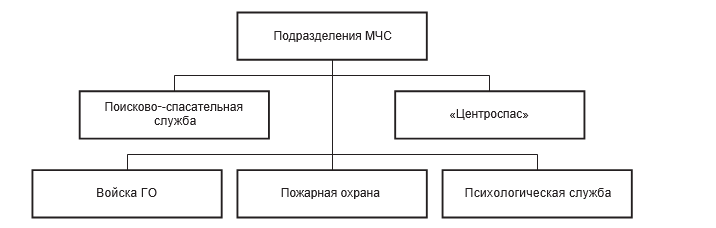
\includegraphics[scale=1]{Pics/1.png}}
\caption{Моделируемые подразделения МЧС}
\label{1}
\end{figure}

\begin{figure}
\center{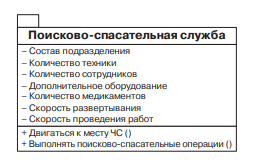
\includegraphics[scale=1]{Pics/2.png}}
\caption{Диаграмма модели поисково-спасательной
службы}
\label{2}
\end{figure}

\begin{figure}
\center {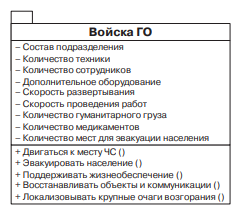
\includegraphics[scale=1]{Pics/3.png}}
\caption{Диаграмма модели войск ГО}
\label{3}
\end{figure}

\begin{figure}
\center {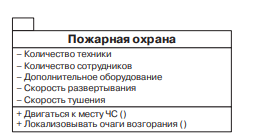
\includegraphics[scale=1]{Pics/4.png}}
\caption{Диаграмма модели пожарной охраны}
\label{4}
\end{figure}

\begin{figure}
\center {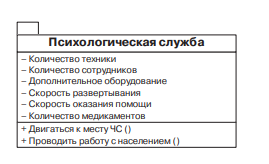
\includegraphics[scale=1]{Pics/5.png}}
\caption{Диаграмма модели психологической службы}
\label{5}
\end{figure}

\begin{figure}
\center {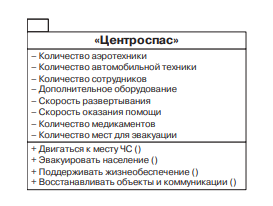
\includegraphics[scale=1]{Pics/6.png}}
\caption{Диаграмма модели «Центроспас»}
\label{6}
\end{figure}


Необходимость описания данных моделей в виде
групповых объектов обусловлена тем, что в реальных
системах, для которых строятся указанные имитационные модели, взаимодействие осуществляется не отдельными единицами, а объединенными группами. Соответственно рассмотрение и моделирование подобных
систем должно осуществляться в контексте взаимодействия групповых объектов. В противном случае могут
быть не учтены какие-либо важные и значимые
свойства.
Моделируемые единицы представляют собой элементы подразделений, участвующих в операциях. Это
может быть колесная или гусеничная техника, летательные аппараты, стационарные единицы, расчеты
и т. д. Каждый подобный элемент имеет ряд характеристик, в частности тип элемента, назначение элемента,
функциональные возможности, технические характеристики, степень работоспособности и т. д. Элемент
группового объекта представляет собой модель физического объекта. В общем случае он может быть охарактеризован следующей совокупностью:

\[E_{i}=\langle X_{i}Y_{i}Z_{i} H_{i}G_{i} \rangle \]

 где
\[X_{i}=\{ x_{j}|j = \overline{1,NX}\}\]
 — множество входных сигналов элемента;
\[Y_{i}=\{ y_{j}|j = \overline{1,NY}\}\]
множество выходных сигналов элемента ;
\[Z_{i}=\{ z_{j}|j = \overline{1,NZ}\}\]
 — множество состояний элемента;
\[H_{i}=\{ h_{j}|j = \overline{1,NH}\}\]
 — множество параметров элемента
(в соответствии с диаграммами); 
\[G_{i}=\{ g_{j}|j = \overline{1,NG}\}\]
— множество функций элемента.
Очевидно, что построение моделей подразделений,
состоящих из подобных элементов, связано с моделированием однотипных единиц, обладающих общими
свойствами. Это дает возможность при построении моделей объединять элементы в групповые объекты, повышая эффективность создания и управления отдельными единицами.
Групповой объект может быть охарактеризован как
множество GO независимо функционирующих однородных элементов Ei
, связанных коммуникационной
функцией F:

\[
GO = \{ E_{i}|i = \overline{1,N}\}
\]
\[
F \subset  \Bigg( \bigcup_{i=1}^{N}Y_{i}       \Bigg)  \times \Bigg( \bigcup_{i=1}^{N}X_{i}  \Bigg), 
\]

причем

\[
\forall y  \in  \Bigg( \bigcup_{i=1}^{N}Y_{i}       \Bigg), x \in  \Bigg( \bigcup_{i=1}^{N}X_{i} \Bigg): yFx
\]

\section{Тестовый код (для примера)}

\begin{lstlisting}
// Hello.java
import javax.swing.JApplet;
import java.awt.Graphics;

public class Hello extends JApplet {
    public void paintComponent(Graphics g) {
        g.drawString("Hello, world!", 65, 95);
    }    
}
\end{lstlisting}
\section{Описание функций}
Функция F связывает элементы Ei
 между собой, обеспечивая передачу информации с выходов одних элементов на входы других.
Групповой объект любой структуры и сложности может быть единообразно описан в виде агрегативной системы или A-схемы, агрегатами Ai
 (рис. ~\ref{7}) которой являются элементы Ei.

Функционирование агрегата в момент времени 

\[
t \in T  \Bigg( T = \{t_{j} |j= \overline{1,NT} \}  \Bigg)
\]

описывается состоянием, входными
сигналами, выходными откликами и внутренними параметрами: 

\[
z(t) \in Z, x(t) \in X, y(t) \in Y, h(t) \in H
\]
Переход агрегата из состояния

\[
z_{j}(t_{i})
\]
в состояние
\[
z_{k}(t_{i+1}) (j \neq k) 
\]
зависит  от h(t) и x(t),переход происходит за малый интервал времени

\begin{figure}
\center {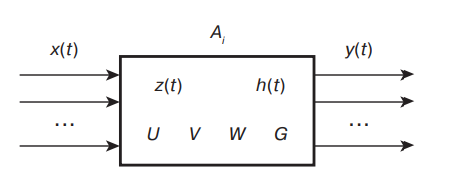
\includegraphics[scale=1]{Pics/7.png}}
\caption{Агрегат ${A_i}$}
\label{7}
\end{figure}


При поступлении сигнала ${x_m}$ в момент времени ${t_m}$
m состояние агрегата определяется с помощью оператора V:


\[
z(t_{m}+0) = V[t_{m},x_{m},z(t_{m})],
\]
где
\[
t = t_{m} +0
\]
момент времени t принадлежит бесконечно малому полуоткрытому интервалу
\[
 t  \in (t_{m},t_{n}].
\]
Рассмотрим интервал времени  $({t_m},{t_m+1})$.Если он не
содержит моментов поступления сигналов, то для момента времени $t \in ({t_m},{t_m+1})$ состояние агрегата определяется оператором U:
\[
z(t) = U[t,t_{m}, z(t_{m}+0)]
\]
Особые состояния агрегата, возникающие в момент
времени ${t_s}$ при поступлении входных сигналов, обозначим через $z({t_s})[1]$. Смену состояний в моменты времени ${t_s}$ обозначим через оператор W :
\[
z(t_{s}+0) = W[t_{s}, z(t_{s})]
\]
Выдача выходных откликов определяется с помощью оператора выхода J:
\[
y(t_{s}) = J[t_{s}, z(t_{s}+0)]
\]
Таким образом, каждый агрегат Ai
 задается совокупностью вида
\[
A_{i}=\langle X,H,Z,Y,U,V,W,J \rangle 
\]
За счет универсального описания применение
A-схемы позволяет охарактеризовывать любые групповые объекты в отрыве от контекста их функционирования и использования. Формальное описание отдельных $\footnote{Тут могла быть ваша сноска}$
агрегатов может быть уточнено путем введения типовых математических схем, позволяющих конкретизировать функционирование элементов агрегативной системы. Наиболее эффективно функционирование агрегатов группового объекта описывается в виде конечного
автомата или сети Петри.

Конечный автомат или F-схема типового агрегата
задается конечными множествами $XF=\{{x_0},{x_1},{x_2},{x_3},\}$ —
множество входных воздействий (${x_0}$ — работать в нормальном режиме; ${x_1}$
 — останов; ${x_2}$— работать в критическом режиме; ${x_3}$ — выход из строя), $YF \subseteq Y$ — множество выходных откликов, $AF=\{ {a_0},{a_1},{a_2},{a_3}\}$ — множество внутренних состояний (${a_0}$
 — функционирование
в нормальном режиме; ${a_1}$
 — останов; ${a_2}$ — функционирование в критическом режиме; ${a_3}$
 — агрегат ${A_i}$ выведен из строя).

Функционирование конечного автомата определяется следующими отображениями [2]:
$\phi : XF\times AF \to  AF$ — переходы автомата;
$\psi : XF\times AF \to  YF$ — выходы автомата.
Таким образом, агрегат ${A_i}$
 представляется в виде
совокупности:
\[
	FA = \langle XF,AF,YF \phi, \psi \rangle
\]
Поскольку в общем случае выдача выходных сигналов агрегатом может осуществляться не только при поступлении сигналов на вход, но и при изменении внутренних параметров. Рассмотрим F-автомат Мура агрегата Ai
, для которого функция выходов определяется
как $y(t) = \psi(z(t))$ (~\ref{10})


\begin{table}
\caption{Переходы F-автомата Мура типового агрегата ${A_i}$}
\center
\begin{tabular}{ || l | l | l | l | l || }

\hline
 & ${y_0}$ & ${y_1}$ & ${y_2}$ & ${y_3}$ \\ \hline
  & ${a_0}$ & ${a_1}$ & ${a_2}$ & ${a_3}$ \\ \hline
 ${x_0}$&${a_0}$ & - & ${a_1}$ & - \\ \hline
${x_1}$&- & ${a_0}$ & ${a_0}$ & -  \\ \hline
${x_2}$&${a_2}$ & ${a_2}$ & - &  -\\ \hline
${x_3}$&${a_3}$ & ${a_3}$ & ${a_3}$& - \\ \hline
\hline
\end{tabular}
\label{10}
\end{table}

Матрица соединений C и вектор выходов $\overrightarrow{y}$
 выглядят следующим образом:


C =
$\begin{pmatrix}
 0 & x_{0} & x_{2} & x_{3} \\
x_{1} & x_{0} &  x_{2} &  x_{3} \\
x_{1} &  x_{0} & 0 &  x_{3} \\
x_{0} &  x_{0} &  x_{0} &  x_{0} 
\end{pmatrix}$

$\overrightarrow{y}$ =
$\begin{pmatrix}
 y_{0} &  \\
y_{1}  \\
y_{2}  \\
y_{3}  
\end{pmatrix}$

На рис. (~\ref{8}) представлен граф переходов и выходов конечного автомата типового агрегата ${A+i}$ .

\begin{figure}
\center {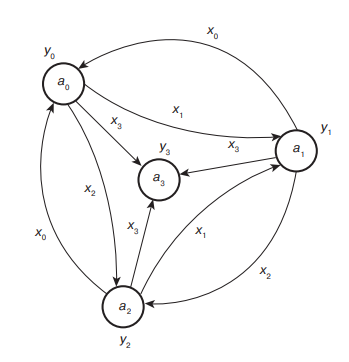
\includegraphics[scale=1]{Pics/8.png}}
\caption{Граф конечного автомата Мура
типового агрегата ${A_i}$}
\label{8}
\end{figure}

Принимая во внимание наличие в системе процессов стохастического характера (например, выход
из строя агрегата ${A_i}$), сигнал ${x_3}$ можно представить в виде случайной величины, определяемой вероятностью
поломки агрегата ${A_i}$.
Формализовать агрегат ${A_i}$ допустимо также с помощью сети Петри или N-схемы.
Сеть Петри агрегата ${A_i}$ задается в виде совокупности
$NA =\langle PN,DN,FN,MN \rangle$, где $PN=\{{p_i}|i=0...{N_PN} -1 \}$
множество мест (позиций) сети;
$DN = \{{d_i}|i=0...{N_DN}-1\}$ - множество переходов сети
$(PN \cap DN  = \emptyset); FN=(PN \times DN) \cup (DN \times PN)$
 — отношения инцидентности сети (дуги графа)

\[
((FN \neq \emptyset) \land (\forall \omega \in PN \cup DN, \upsilon \in PN \cup DN : \omega FN \upsilon \vee \upsilon FN \omega))
\]

Кратность всех дуг сети равна 1;
$MN : PN \rightarrow N $— разметка сети Петри, где  N —
множество натуральных чисел.
Число фишек (меток) в позиции ${p_i}$ задается следующим образом:
\[
\forall p \in PN, MN(p) =n.
\]
Множество MN может быть задано в векторном
виде:
\[
	MN = (MN(p_{0}), MN(p_{1}),...,MN(p_{PN-1}))^T
\]
Начальная разметка сети определяется следующим
образом:
\[
	MN^(0)=(1,0,0,0,0,1,0,0)^T
\]
Позиции ${p_0},{p_1},{p_2},{p_3}$ эквивалентны состояниям
 ${a_0},{a_1},{a_2},{a_3}$ описанного выше конечного автомата. Позиции 3456 pppp ,,, эквивалентны входным сигналам
 ${x_0},{x_1},{x_2},{x_3}$ .
Достоинством сети Петри является возможность
проверить достижимость определенной разметки аналитическим способом.
Двудольный граф сети Петри представлен на рис. 9.
Получив формальное описание агрегатов, можно
построить модель всей агрегативной системы (группового объекта). Для этого необходимо определить структуру A-схемы и характер взаимодействия агрегатов.
Агрегативная система состоит из N агрегатов, называемых полюсами. В зависимости от конкретного группового объекта агрегаты могут являться входными, выходными или внутренними полюсами.
Каждый агрегат ${A_i}$ имеет как входные контакты,
представленные множеством $X^(i)$ , на которые подается
входной алфавит, так и выходные — множество $Y^(i)$ ,
с которых снимается выходной алфавит [3].
Поскольку взаимодействие между агрегативной системой и внешней средой также осуществляется посредством сигналов, внешняя среда может быть представлена в виде агрегата ${A_0}$ . Соответственно на входные
контакты $X^(0)$ будут поступать выходные сигналы агрегативной системы, а с выходных контактов $Y^(0)$ данные
будут идти на входные контакты системы. Взаимодействие агрегатов между собой осуществляется с помощью коммуникационной функции F.
Приведенные реализации группового объекта с применением типовых математических схем аппарата имитационного моделирования положены в основу программных компонент, написанных на языке высокого
уровня и представляющих собой интерфейсы и реализации базовых классов. Разработанные базовые классы
представляют собой шаблоны, опираясь на которые
можно задавать специализацию конкретных групповых
объектов, проводя наследование и реализуя дополнительные функции и методы.
В результате проведенных исследований разработана математическая модель группового объекта на основе A-схемы. Кроме того, формализована агрегативная
система, состоящая из N элементов. Проделанная работа позволила также получить математическое описание
отдельных агрегатов с использованием F- и N-схем.
Разработанная модель группового объекта может
служить основой для построения программных моделей для систем имитационного моделирования ликвидации последствий ЧС.
\begin{figure}
\center {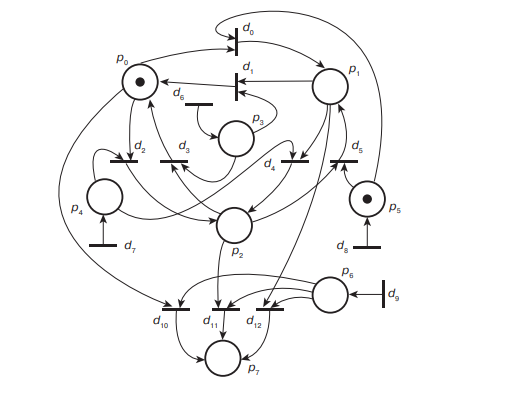
\includegraphics[scale=1]{Pics/9.png}}
\caption{Двудольный граф сети Петри для агрегата ${A_i}$}
\end{figure}


\begin{thebibliography}{99}
\bibitem{1}
Советов Б.Я. Моделирование систем. М.: Высш. шк., 2005.
343 с.: ил.

\bibitem{2} 
Сирота А.А. Компьютерное моделирование и оценка эффективности сложных систем. М.: Техносфера, 2006.
280 с.: ил.

\bibitem{3} 
Бусленко Н.П. Моделирование сложных систем. М.: Наука,
1968. 356 с.: ил.
Федеральный закон от 27 июля 2006 г. N 149-ФЗ "Об информации,
информационных технологиях и о защите информации"


\end{thebibliography}
\end{document}